\documentclass[10pt]{article}
\usepackage{preamble}

\def\FS{Formelsammlung}
\def\Fach{Elektrische Messtechnik 2}
\def\FachAkz{MT2}
\title{\FS \\ \Fach}
\date{\today}
\def\Semester{Sommersemester 2026}

\author{\href{https://github.com/BastianNagler/MT2_Formelsammlung}{Bastian Nagler}}
\def\MatNr{MATNR}

\begin{document}

\pagenumbering{gobble}
\begin{titlepage}
	\thispagestyle{empty}

	\begin{center}
		
\includegraphics[width=0.7\textwidth]{../OTHR_OTHR_Logo}\\
		\vspace*{\stretch{1}}
		\Huge
		\textsc{\MyTitle}\\
		\vspace*{\stretch{0.25}}
		\large
		\textbf{\Semester}\\
		{\small
		nach Vorlesung von Prof. Maier}

		\vspace*{\stretch{0.5}}
		\href{https://github.com/BastianNagler/MT2_Formelsammlung}{Bastian Nagler}


		\vspace*{\stretch{2}}
		{\renewcommand{\arraystretch}{1.5}
			\begin{tabular}{l l}
				Letzte Änderung: & \hspace{4cm}\MyDate   \\
				Lizenz:          & \hspace{4cm}GPLv3
			\end{tabular}
		}
		\vspace*{\stretch{1}}
		\vspace*{\stretch{2}}


	\end{center}
\end{titlepage}

\newpage
\tableofcontents
\clearpage

\pagestyle{fancy}
\lhead{\MyAuthor}
\rhead{\Semester}
\cfoot{\vspace{-20pt}\thepage}
\pagenumbering{arabic}
% \setlength{\columnsep}{1pt}
\raggedcolumns

\begin{multicols*}{2}
	\section{Sensoren}

\subsection{Schalter}
    \begin{itemize}
        \item Vorteile 
            \begin{itemize}
                \item Einfach und Kostengünstig
                \item Hohe Lebensdauer
                \item Hohe Spannungen und Ströme schaltbar
            \end{itemize}
        \item Nachteile 
            \begin{itemize}
                \item Prellen / Kleben
                \item Langsam
            \end{itemize}
    \end{itemize}

    \textbf{Entprellen durch:} 
    
    \begin{minipage}{0.48\columnwidth}
        Tiefpass + Schmitt-Trigger:
        \begin{figure}[H]
            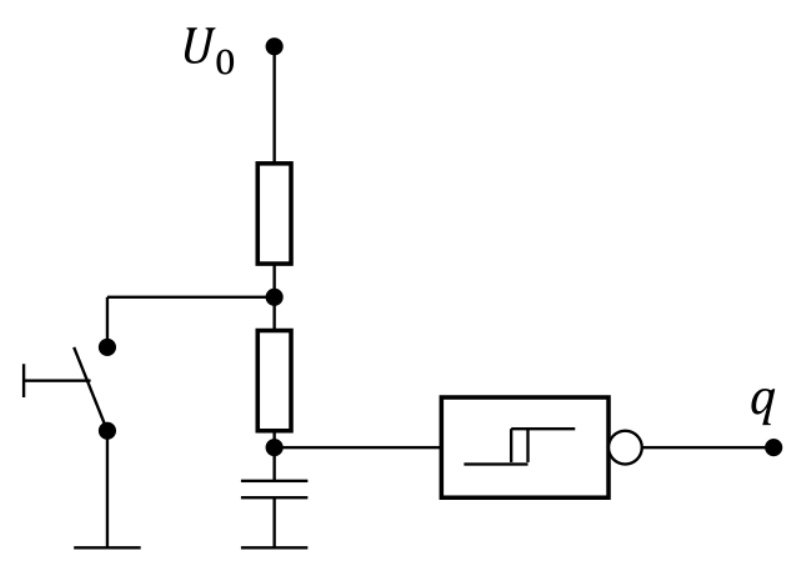
\includegraphics[width=0.98\textwidth]{Figures/sensoren/schalter_schmitt.png}
        \end{figure}
        wobei: \(RC > Prelldauer\)     
    \end{minipage}
    \hfill
    \begin{minipage}{0.48\columnwidth}
        Verriegelungsschaltung:
        \begin{figure}[H]
            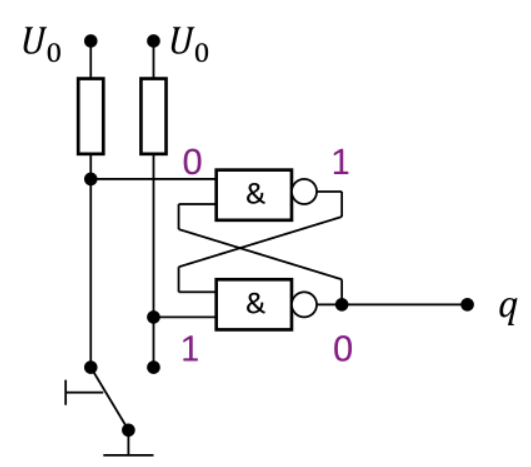
\includegraphics[width=0.98\textwidth]{Figures/sensoren/schalter_verriegelung.png}
        \end{figure}    
    \end{minipage}

\subsubsection{Lichtschranke}
    \begin{itemize}
        \item Vorteile 
            \begin{itemize}
                \item Berührungslos, keine Rückwirkung auf Messobjekt
                \item Sehr hohe Lebensdauer, verschleißfrei
                \item relativ Kostengünstig
                \item Hohe Schaltgeschwindigkeit
            \end{itemize}
        \item Nachteile 
            \begin{itemize}
                \item Lichtweg darf nicht gestört werden (Absorption, Streuung)
                \item Störlichtquellen (Sonne, andere Lampen)
            \end{itemize}
    \end{itemize}

\subsection{Winkel- und Längenmessung}
    \subsubsection{Potentiometer}
        \begin{figure}[H]
            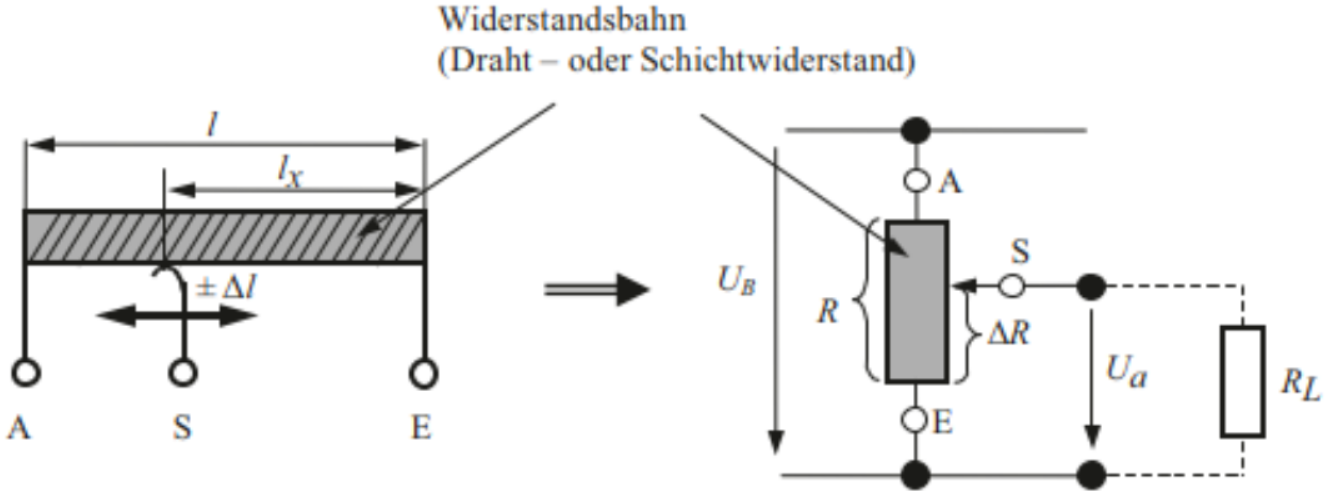
\includegraphics[width=0.9\columnwidth]{Figures/sensoren/poti_schiebe.png}
        \end{figure}
        \begin{align*}
            U_a &= U_B \cdot \frac{\Delta R}{R} \\
            \Aboxed{
                U_a &= U_B \cdot \frac{l_x}{l} = U_B \frac{\alpha}{\alpha_0}
            }
        \end{align*}
        \textbf{Bei Belastung des Spannungsteilers wird der Messwert verfälscht}

    \subsubsection{Inkrementalgeber}
        \begin{figure}[H]
            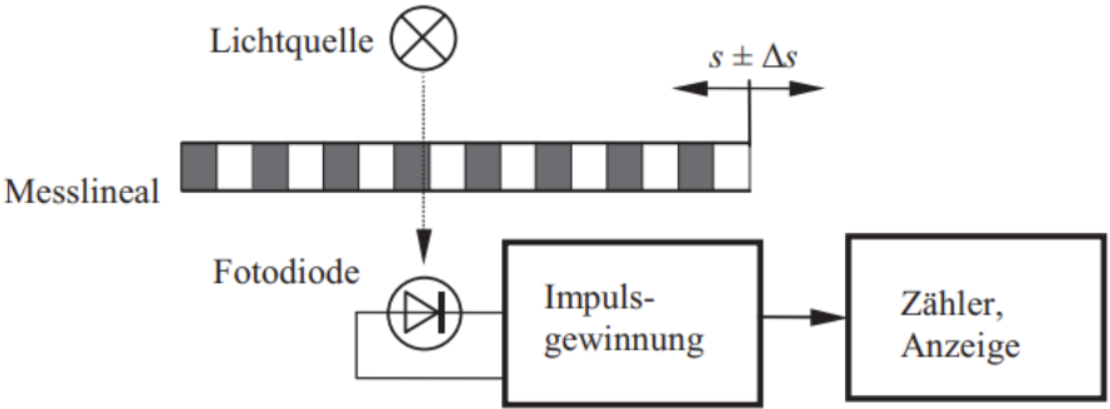
\includegraphics[width=0.9\columnwidth]{Figures/sensoren/inkrementalgeber.png}
        \end{figure}
        \begin{itemize}
            \item Messprinzip 
                \begin{itemize}
                    \item Zählung der hell/dunkel Phasen der Fotodiode
                    \item Die Längenauflösung beträgt \(\Delta s\) (1 Periode des Messlineals)
                \end{itemize}
            \item Vorteile 
                \begin{itemize}
                    \item relativ einfach
                    \item Sensor berührungslos
                \end{itemize}
            \item Nachteile 
                \begin{itemize}
                    \item Hier keine Richtungserkennung möglich
                    \item Keine absolute Positionsmessung
                    \item Für abs. Position muss bekannte Referenzposition angefahren werden.
                    \item Synchronisation der Bitwechsel bei 2 Messlinealen \textrightarrow Gray-Code
                    {\small
                        Generierung Gray-Code\\
                        X1: Dualzahl im Binärcode\\
                        X2: X1 >> 1 (Rechtsshift um 1)\\
                        Gray-Code X3: X1 xor X2
                    }
                \end{itemize}
        \end{itemize}

        \textbf{Verbesserung durch 2 Messlineale, welche } \(\frac{\Delta s}{4}\) \textbf{verschoben sind.}
        {\footnotesize s. Sensoren S. 17}

        Drehzahlmessung:
        \begin{itemize}
            \item Zählung der Impulse \(N\) in fester Zeit \(T\): \\
                \(\omega = \frac{\Delta \varphi \cdot N}{T}\) \\ 
                Auflösung: \(\Delta \omega = \frac{\Delta \varphi}{T}\)
            \item Messung der Zeitdifferenz zwischen zwei folgenden Pulsen: \\
                \(\omega = \frac{\Delta \varphi}{T}\) \\
                Auflösung: \(\Delta \omega = \frac{\Delta \varphi}{T^2} \cdot \Delta T\)
        \end{itemize}
    
\subsection{Temperaturmessung}
    \subsubsection{Widerstände}
        \begin{itemize}
            \item Pt100: Platin-Widerstandsthermometer mit 100 \(\Omega\) bei 0 °C
            \item Pt1000: Platin-Widerstandsthermometer mit 1000 \(\Omega\) bei 0 °C (Vorteil: Geringerer Fehler durch Leitungswiderstand)
        \end{itemize}
        \begin{align*}
            R(\vartheta) &= R_0 \cdot (1 + \alpha \cdot (\vartheta - \vartheta_0) + \beta (\vartheta - \vartheta_0)^2 + \ldots) \\
            R(\vartheta) &\approx R_0 \cdot (1 + \bar{\alpha} \cdot (\vartheta - \vartheta_0)) \text{ mit } \bar{\alpha} = \frac{R(\vartheta_1) - R(\vartheta_0)}{R(\vartheta_0) \cdot (\vartheta_1 - \vartheta_0)}\\
            &\text{Platin: } \bar{\alpha} \approx 3850 \cdot 10^{-6} \frac{1}{^\circ C}
        \end{align*}
        Auswertung durch Widerstandsmessung: 
        \begin{itemize}
            \item Zweileiter-Messung: \(R_{gemessen} = R_{Pt} + 2 \cdot R_{Leitung}\)
            \item Vierleiter-Messung: \(R_{gemessen} = R_{Pt}\)
        \end{itemize}
        Ansprechzeit: \(t_{0,5}\) bzw. \(t_{0,9}\) Zeit, nach der 50\% bzw. 90\% des Endwerts erreicht sind. (Sprunganregung)\\
        Selbsterwärmung mit Selbsterwärmungskoeffizient \(S\): \(\Delta T = S \cdot P\)
    \subsubsection{Thermodiffusion/Seebeck}
        \begin{itemize}
            \item Benötigen Vergleichstemperatur
            \item Einsatz bei sehr hohen Temperaturen
            \item Ungenauer als Pt100, aber schnelleres Ansprechverhalten
        \end{itemize}
        \begin{figure}[H]
            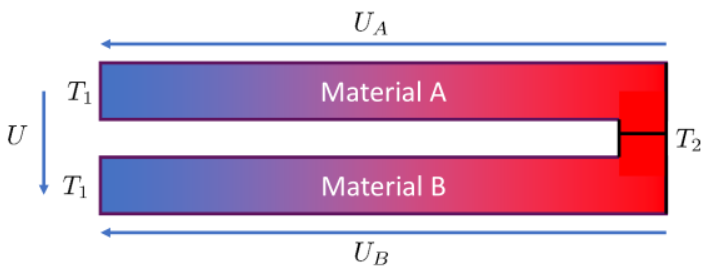
\includegraphics[width=0.9\columnwidth]{Figures/sensoren/thermodiffusion.png}
        \end{figure}
        \begin{align*}
            U \approx (S_B - S_A) \cdot (T_2 - T_1)
        \end{align*}
    \subsubsection{NTC}
        \begin{align*}
            R(\vartheta) = R_0 \cdot e^{B \cdot (\frac{1}{T} - \frac{1}{T_0})} \text{Achtung in Kelvin}
        \end{align*}

\subsection{Kraftmessung}
    \subsubsection{DMS}
        \begin{align*}
            \frac{\Delta R}{R} = \left( \frac{\Delta \rho}{\rho \varepsilon} + 2 \mu + 1 \right) \cdot \varepsilon = k \cdot \varepsilon
        \end{align*}
        \begin{itemize}
            \item Halbleiter-DMS:
                \begin{itemize}
                    \item Sehr hoher \(k\)-Faktor, für hohe Empfindlichkeit
                    \item Stärkere und nichtlineare Temperaturabhängigkeit
                    \item Nichtlinear bei großen Dehnungen
                \end{itemize}
            \item Metall-DMS:
                \begin{itemize}
                    \item Geringerer \(k\)-Faktor (\(\approx 2\))
                    \item lineare Temperaturabhängigkeit
                    \item Linear bei großen Dehnungen
                \end{itemize}
        \end{itemize}
        Messwertverarbeitung:
        \begin{itemize}
            \item Viertelbrücke: \\
                \(U_{AB} \approx \frac{\Delta R}{4R} \cdot U_0 = \frac{U_0}{4} \cdot k \cdot \varepsilon\)
            \item Halbbrücke (unbelasteter Balken): \\
                \(U_{AB} \approx \frac{\Delta R}{4R} \cdot U_0 = \frac{U_0}{4} \cdot k \cdot \varepsilon\) \\
                Vorteil: Temperaturkompensation, da beide DMS die gleiche Temperatur haben
            \item Halbbrücke (selber Balken): \\
                \(U_{AB} \approx \frac{\Delta R}{2R} \cdot U_0 = \frac{U_0}{2} \cdot k \cdot \varepsilon\) \\
                Vorteil: Höhere Empfindlichkeit, Temperaturkompensation (DMS an unterschiedlichen Seiten des Balkens)
            \item Vollbrücke: \\
                \(U_{AB} \approx \frac{\Delta R}{R} \cdot U_0 = U_0 \cdot k \cdot \varepsilon\)
        \end{itemize}

    \subsubsection{Piezoeffekt}
        Ladung direkt proportional zur auf den Sensor wirkenden Kraft:
        \begin{align*}
            Q = k_p \cdot F
        \end{align*}
        \begin{figure}[H]
            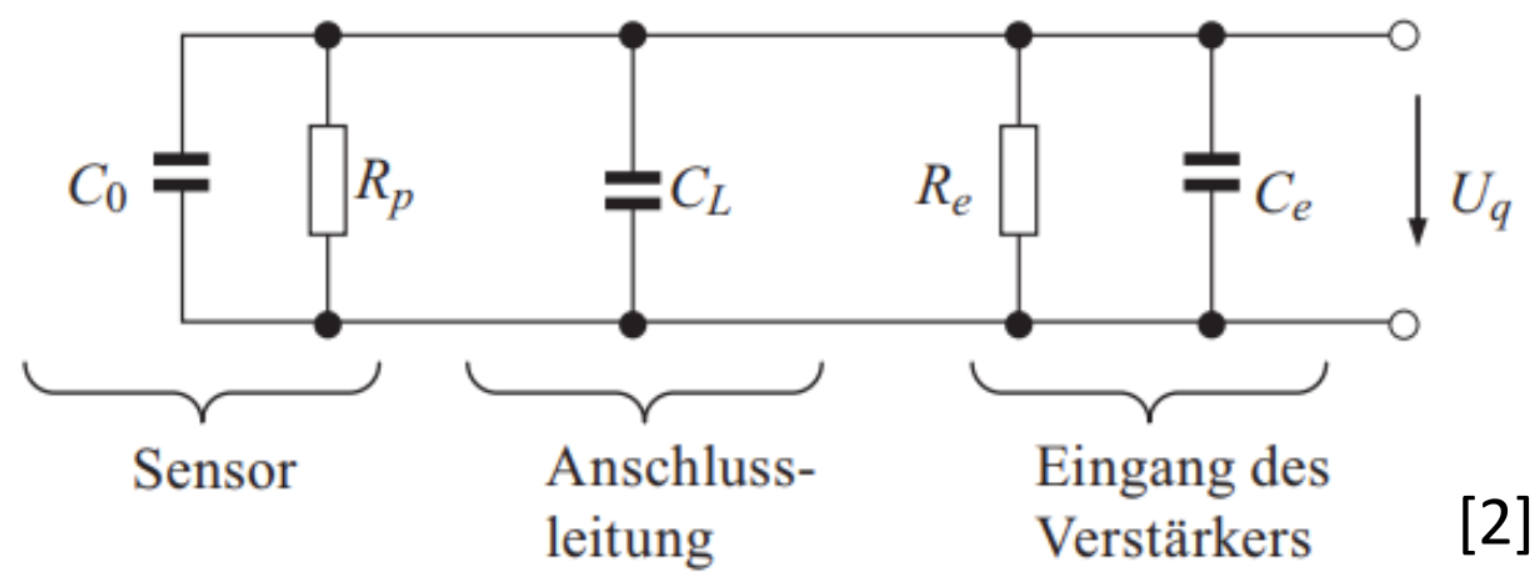
\includegraphics[width=0.9\columnwidth]{Figures/sensoren/piezo_basic.png}
        \end{figure}
        \begin{align*}
            U_q = \frac{Q}{C_{ges}} = \frac{k_p \cdot F}{C_0 + C_L + C_e}
        \end{align*}
        Probleme:
        \begin{itemize}
            \item Messaufbau verändert Empfindlichkeit
            \item Widerstände müssen sehr hoch sein, um Ladung nicht zu entladen (Wertänderung über Zeit, da \(\tau = R_{ges} \cdot C_{ges}\))
        \end{itemize}
        \textrightarrow Messung von veränderlichen Kräften

        \textbf{Ladungsverstärker}
        \begin{figure}[H]
            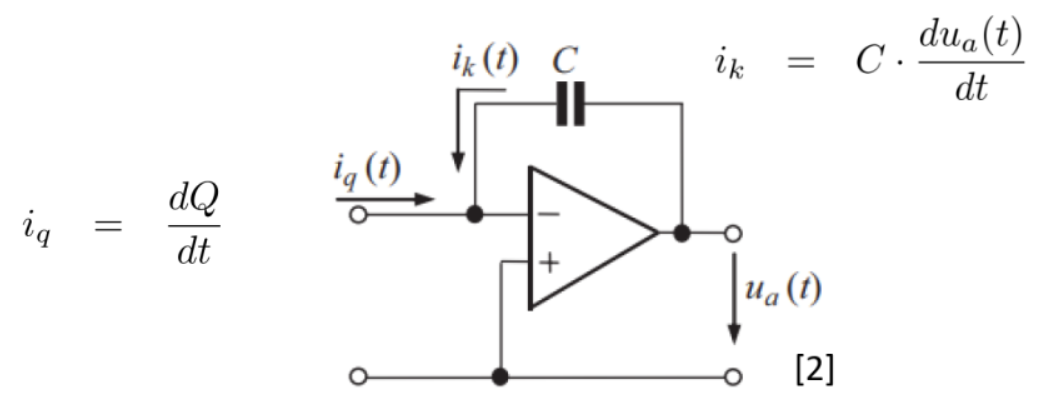
\includegraphics[width=0.9\columnwidth]{Figures/sensoren/piezo_ladungsverst.png}
        \end{figure}
        \begin{align*}
            u_a(t) = - \frac{Q}{C} = - \frac{k_p \cdot F(t)}{C}
        \end{align*}
        \begin{itemize}
            \item Ausgangsspannung unabhängig von parasitären Kapazitäten
            \item Messbereichsanpassung durch Wahl von \(C\)
            \item Entladen von C vor Messung notwendig
        \end{itemize}

\subsection{Druckmessung}
    \begin{align*}
        h &= \frac{T_0}{k_T} \cdot \left[ 1 - \left( \frac{p}{p_0} \right)^{-\frac{k_T R_s}{g}} \right] + h_0 \\
          & \approx 44.300m \cdot \left[ 1 - \left( \frac{p}{p_0} \right)^{-0,1903} \right] + h_0 \\
        S &= \frac{\partial h}{\partial p} = - 8,32 \frac{\mathrm{m}}{\mathrm{hPa}}
    \end{align*}
    Bei konstanter Temperatur (isotherm):
    \begin{align*}
        h = h_0 - \frac{R \cdot T}{M \cdot g} \cdot \ln \left( \frac{p}{p_0} \right)
    \end{align*}
	\clearpage

	\section{OpAmp}
\subsection{Realer OpAmp}
    \begin{table}[H]
        \begin{tabular}{l l r r}
            \toprule
            Symbol & Erklärung & Ideal & Real \\
            \midrule
            \(V_0\) & Verstärkung & \(\infty\) & \(10^5..10^8\) \\
            \(V_{Gl}\) & Gleichtaktvers. & \(0\) & \(0,1..0,3\) \\
            \(r_E\) & AC Eingangs-R & \(\infty\) & \(10^7..10^12 \mathrm{\Omega}\) \\
            \(r_{gl}\) & DC Eingangs-R & \(\infty\) & \(r_{gl} > r_E\) \\
            \(I_{P0}, I_{N0}\) & Eingangsstrom & \(0\) & \(0,1..25 \mathrm{nA}\) \\
            Slew Rate &  & \(\infty\) & \(0,5..1000 \mathrm{\frac{V}{\mu s}}\) \\
            \(U_{D0}\) & Offsetspannung & \(0\) & \(0,1..5 \mathrm{mV}\) \\
            \bottomrule
        \end{tabular}
    \end{table}

    \vspace{-16pt}

    \begin{gather*}
        I_{P0} = I_{B+} \quad I_{N0} = I_{B-} \\
        I_B = \frac{I_{B+} + I_{B-}}{2} \\
        I_{OS} = I_{B+} - I_{B-}
    \end{gather*}

\subsection{Grundschaltungen}

    \subsubsection{Invertierender Verstärker}
        \noindent
        \begin{minipage}{0.5\columnwidth}
            \centering
            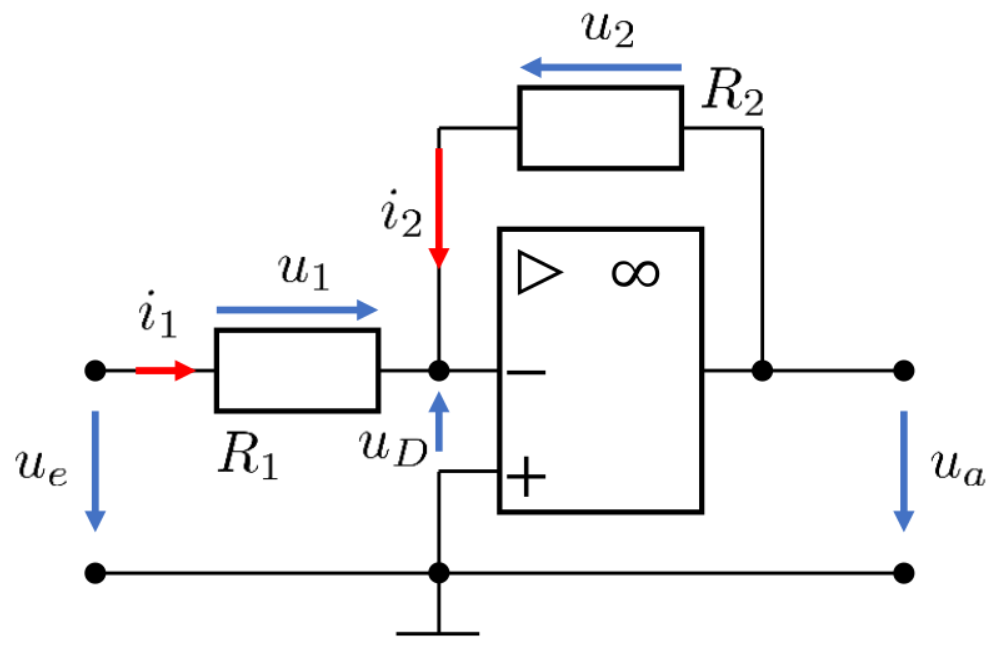
\includegraphics[width=\linewidth]{Figures/opamp/invertingamp.png}
        \end{minipage}%
        \hfill
        \begin{minipage}{0.45\columnwidth}
            \begin{flalign*}
                & u_a = - \frac{R_2}{R_1} \cdot u_e &
            \end{flalign*}
        \end{minipage}
        \vspace{10pt}
    
    \subsubsection{Nicht-Invertierender Verstärker}
        \noindent
        \begin{minipage}{0.5\columnwidth}
            \centering
            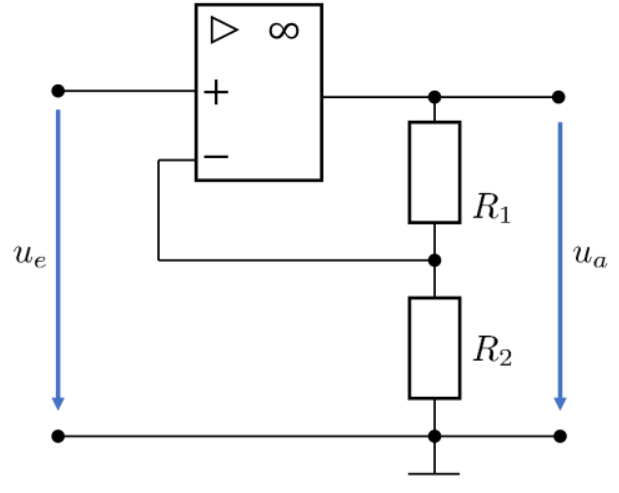
\includegraphics[width=\linewidth]{Figures/opamp/noninvertingamp.png}
        \end{minipage}%
        \hfill
        \begin{minipage}{0.45\columnwidth}
            \begin{flalign*}
                & u_a = \left(1 + \frac{R_1}{R_2} \right) \cdot u_e &
            \end{flalign*}
        \end{minipage}
        \vspace{10pt}

    \subsubsection{Invertierender Addierer}
        \vspace{-10pt}
        \begin{figure}[H]
            \centering
            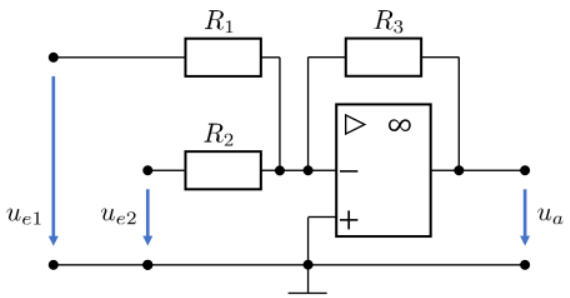
\includegraphics[width=0.6\columnwidth]{Figures/opamp/invertingadder.png}
        \end{figure}
        \vspace{-10pt}
        \begin{align*}
            u_a = - R_3 \cdot \left(\frac{u_{e1}}{R_1} + \frac{u_{e2}}{R_2} \right)
        \end{align*}

    \subsubsection{Subtrahierer}
        \vspace{-10pt}
        \begin{figure}[H]
            \centering
            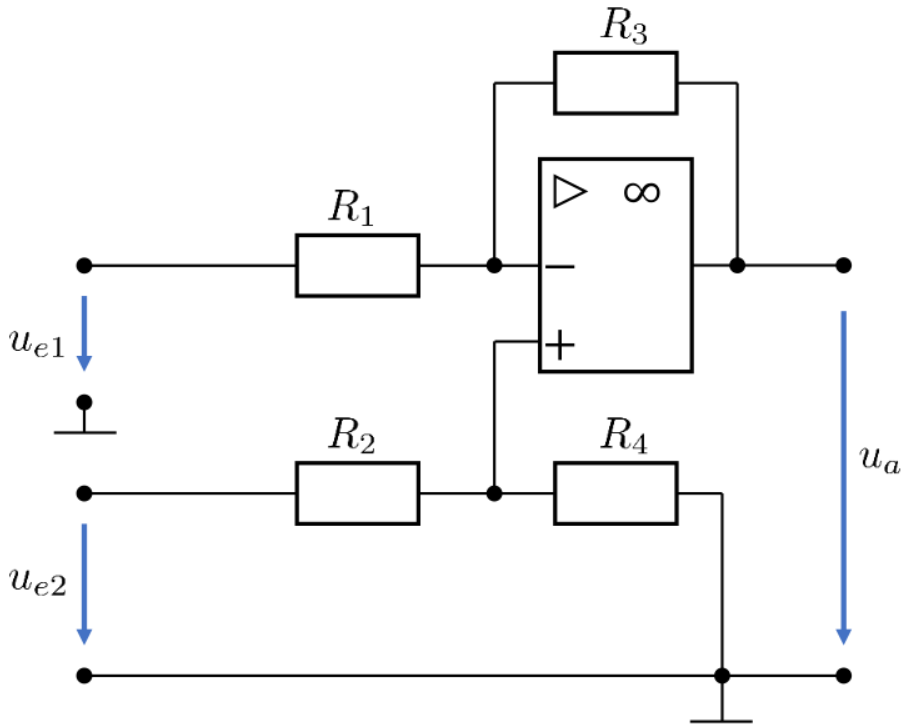
\includegraphics[width=0.6\columnwidth]{Figures/opamp/subtractor.png}
        \end{figure}
        \vspace{-10pt}
        \begin{align*}
                u_a &= \frac{R_4 (R_1 + R_3)}{R_1 (R_2 + R_4)} u_{e2} - \frac{R_3}{R_1} u_{e1} \\
                u_a &= \frac{R_3}{R_1} (u_{e2} - u_{e1}) \qquad \text{wenn} \quad \frac{R_1}{R_3} = \frac{R_2}{R_4}
        \end{align*}

        \textbf{Alternative 1: }
        \vspace{-10pt}
        \begin{figure}[H]
            \centering
            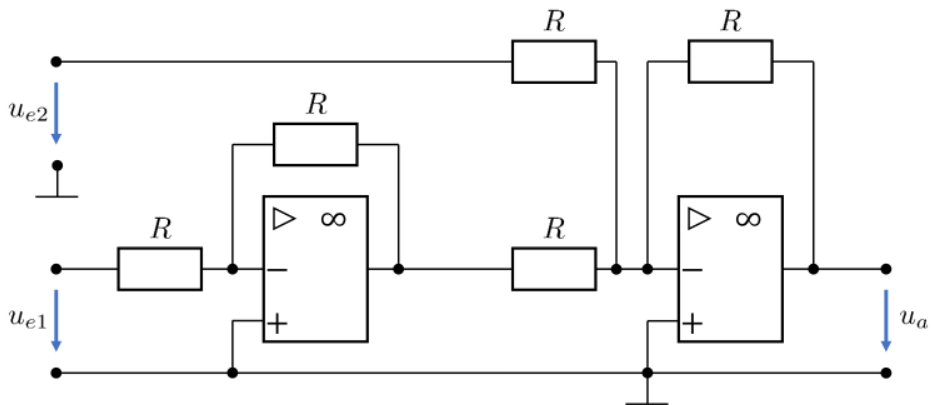
\includegraphics[width=0.7\columnwidth]{Figures/opamp/subtractor_alternative.png}
        \end{figure}
        \vspace{-10pt}
        Aufbau aus Invertierer + Invertierender Addierer
        \begin{align*}
            & u_a = u_{e1} - u_{e2} &
        \end{align*}

        \textbf{Alternative 2: }\\
        \noindent
        \begin{minipage}{0.4\columnwidth}
            \centering
            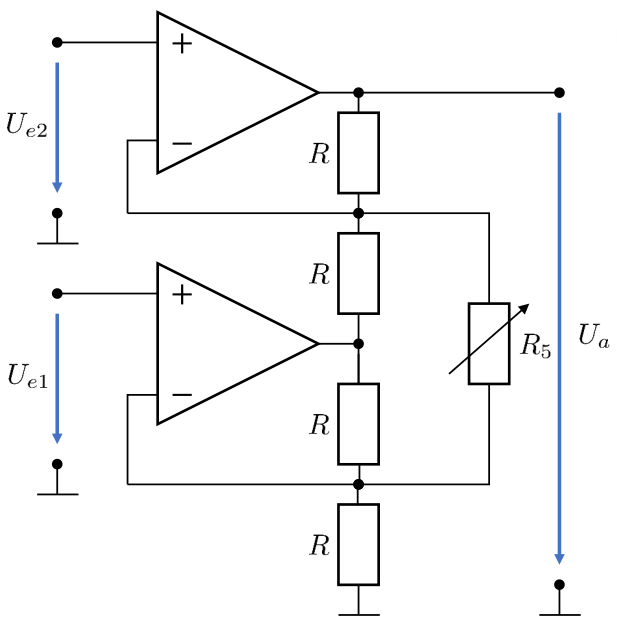
\includegraphics[width=\linewidth]{Figures/opamp/subtractor_alternative2.png}
        \end{minipage}%
        \hfill
        \begin{minipage}{0.55\columnwidth}
            \raggedright
            \begin{flalign*}
                & u_a = 2 \cdot \left( 1 + \frac{R}{R_5} (u_{e2} - u_{e1}) \right) &
            \end{flalign*}
            {\small Vorteil: Nur ein Widerstand zur Einstellung der Verstärkung}
        \end{minipage}
        \vspace{10pt}

    \subsubsection{Integrierer}
        \noindent
        \begin{minipage}{0.4\columnwidth}
            \centering
            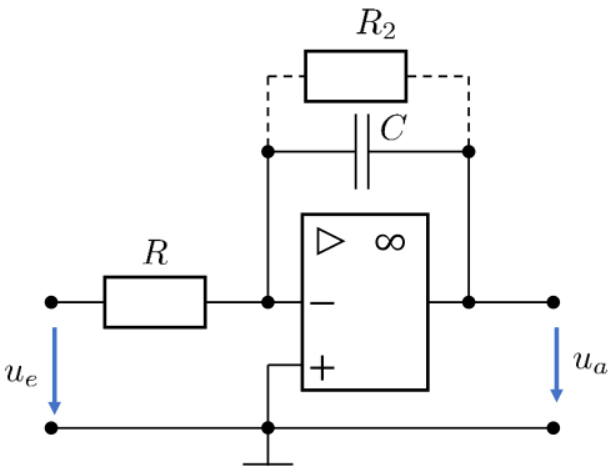
\includegraphics[width=\linewidth]{Figures/opamp/integrator.png}
        \end{minipage}%
        \hfill
        \begin{minipage}{0.55\columnwidth}
            \begin{flalign*}
                & u_a = - \frac{1}{RC} \int_{0}^{t} u_e(t) dt + u_a(0) &
            \end{flalign*}
        \end{minipage}
        \vspace{15pt}

        \textbf{Spezialfall: Ladungsverstärker} (\(R = 0\))\\
        \noindent
        \begin{minipage}{0.45\columnwidth}
            \centering
            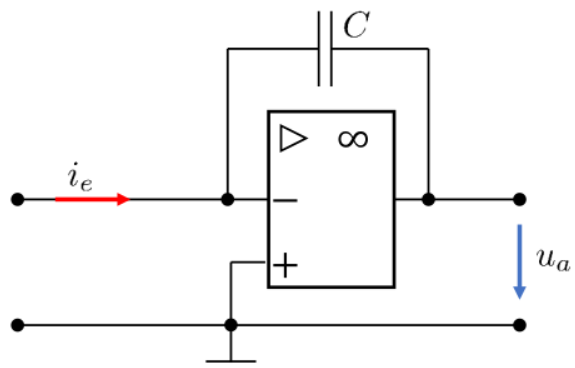
\includegraphics[width=\linewidth]{Figures/opamp/chargeamp.png}
        \end{minipage}%
        \hfill
        \begin{minipage}{0.55\columnwidth}
            \begin{flalign*}
                & \begin{aligned}
                    u_a &= - \frac{1}{C} \int_{0}^{t} i_e(t) dt + u_a(0) \\
                        &= \frac{-q(t)}{C} + u_a(0)
                \end{aligned} &
            \end{flalign*}
        \end{minipage}
        \vspace{10pt}

    \subsubsection{Differenzierer}
        \noindent
        \begin{minipage}{0.4\columnwidth}
            \centering
            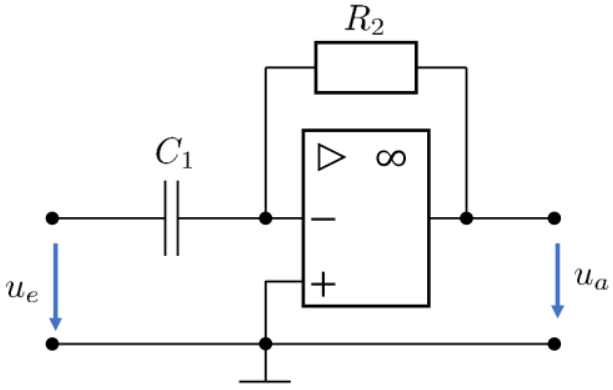
\includegraphics[width=\linewidth]{Figures/opamp/differentiator.png}
        \end{minipage}%
        \hfill
        \begin{minipage}{0.55\columnwidth}
            \raggedright
            \begin{flalign*}
                & U_a (\omega) = - j \omega \cdot R_2 C_1 \cdot U_e(\omega) &
            \end{flalign*}
            \small Schaltung neigt stark zum Schwingen.
        \end{minipage}
        \vspace{15pt}

        \textrightarrow \textbf{Realisierung} (D + PT2-Glied)\\
        \vspace{-10pt}
        \begin{figure}[H]
            \centering
            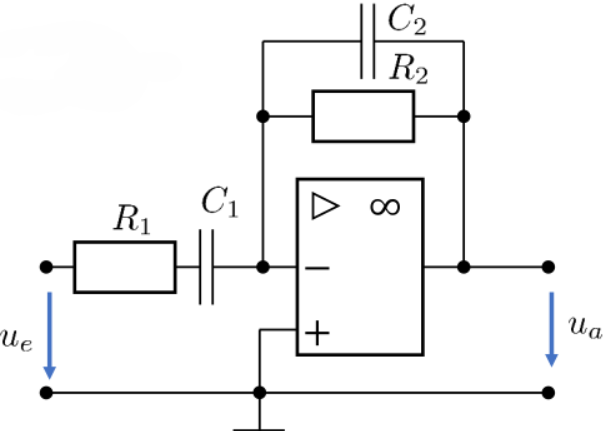
\includegraphics[width=0.5\columnwidth]{Figures/opamp/differentiator_real.png}
        \end{figure}
        \vspace{-10pt}
        \begin{align*}
            & U_a (\omega) =  \frac{ - j \omega \cdot R_2 C_1 \cdot U_e(\omega) }{(1 + j \omega R_1 C_1) \cdot (1 + j \omega R_2 C_2)} &
        \end{align*}

    \subsubsection{Transistor im Rückkopplungspfad}

    
	\clearpage
	//insert Kennlinien
	\clearpage

	\section{Zufällige Messfehler}

\subsection{Allgemeine Definitionen}
    \begin{itemize}
        \item \textbf{Wahrscheinlichkeitsdichtefunktion $f_X(x)$}: Beschreibt die Verteilung der Wahrscheinlichkeiten. Die Fläche unter der Kurve ist immer exakt 1.
        \item \textbf{Verteilungsfunktion $F_X(x)$}: Das Integral der Dichtefunktion. Sie gibt die Wahrscheinlichkeit $P$ an, dass ein Messwert kleiner als ein bestimmtes $x$ ausfällt ($P(X < x)$).
        \item \textbf{Mittelwert (1. Moment) $\mu$}: Der erwartete Wert (Schwerpunkt der Dichtefunktion).
        \begin{align*}
            \mu = E\{X\} = \int_{-\infty}^{\infty} x \cdot f_X(x) \, dx
        \end{align*}
        \item \textbf{n-tes Moment}:
        \begin{align*}
            E\{X^n\} = \int_{-\infty}^{\infty} x^n \cdot f_X(x) \, dx
        \end{align*}
        Für diskrete Werte (z.B. Würfel) werden Integrale zu Summen und die Dichte zur jeweiligen Wahrscheinlichkeit $P(x_i)$ (z.B. $\mu = \sum x_i P(x_i)$).
        \item \textbf{Varianz (2. zentrales Moment) $\sigma^2$}: Beschreibt die mittlere quadratische Abweichung vom Mittelwert. 
        \begin{align*}
            \sigma^2 &= E\{(X - \mu)^2\} = \int_{-\infty}^{\infty} (x - \mu)^2 \cdot f_X(x) \, dx \\
            \sigma^2 &= E\{X^2\} - \mu^2
        \end{align*}
        \item \textbf{Standardabweichung $\sigma$}:
        \begin{align*}
            \sigma = \sqrt{E\{X^2\} - \mu^2}
        \end{align*}
    \end{itemize}

\subsection{Wichtige Verteilungen}

    \subsubsection{Gleichverteilung (Rechteckverteilung)}
        \textbf{Vorkommen:} Alle Werte sind gleich wahrscheinlich. z.B. Quantisierungsfehler.
        \begin{center}
        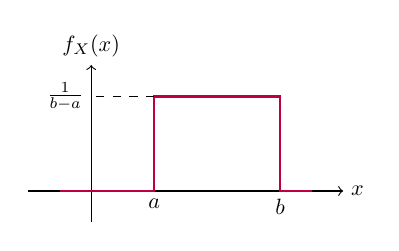
\begin{tikzpicture}[scale=0.8, transform shape]
            \draw[->] (-1,0) -- (4,0) node[right] {$x$};
            \draw[->] (0,-0.5) -- (0,2) node[above] {$f_X(x)$};
            \draw[thick, purple] (-0.5,0) -- (1,0) -- (1,1.5) -- (3,1.5) -- (3,0) -- (3.5,0);
            \draw[dashed] (1,1.5) -- (0,1.5) node[left] {$\frac{1}{b-a}$};
            \node[below] at (1,0) {$a$};
            \node[below] at (3,0) {$b$};
        \end{tikzpicture}
        \end{center}

        \begin{align*}
            \mu = \frac{a+b}{2} \qquad \qquad \sigma^2 = \frac{(b-a)^2}{12} \qquad \qquad \sigma = \frac{b-a}{\sqrt{12}}
        \end{align*}

    \subsubsection{Dreiecksverteilung}
        \textbf{Vorkommen:} Entsteht durch Faltung (Summe) von zwei unabhängigen Gleichverteilungen. (Zwei Würfel) 
        \begin{center}
        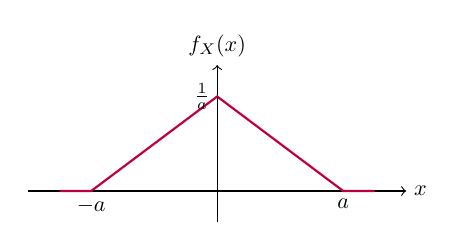
\begin{tikzpicture}[scale=0.8, transform shape]
            \draw[->] (-3,0) -- (3,0) node[right] {$x$};
            \draw[->] (0,-0.5) -- (0,2) node[above] {$f_X(x)$};
            \draw[thick, purple] (-2.5,0) -- (-2,0) -- (0,1.5) -- (2,0) -- (2.5,0);
            \draw[dashed] (0,1.5) -- (0,0);
            \node[left] at (0,1.5) {$\frac{1}{a}$};
            \node[below] at (-2,0) {$-a$};
            \node[below] at (2,0) {$a$};
        \end{tikzpicture}
        \end{center}

        \begin{align*}
            \mu = 0 \qquad \qquad \sigma^2 = \frac{a^2}{6}
        \end{align*}

    \subsubsection{Normalverteilung (Gauss-Verteilung)}
        \textbf{Entstehung \& Vorkommen:} Viele unabhängige Einzelfehler, die sich aufsummieren (Zentraler Grenzwertsatz).
        \begin{center}
        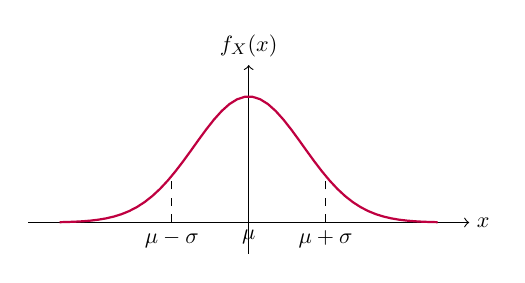
\begin{tikzpicture}[scale=0.8, transform shape]
            \draw[->] (-3.5,0) -- (3.5,0) node[right] {$x$};
            \draw[->] (0,-0.5) -- (0,2.5) node[above] {$f_X(x)$};
            % draw gaussian: e^(-x^2/1.5) * 2
            \draw[thick, purple, domain=-3:3, samples=50] plot (\x, {2*exp(-(\x*\x)/1.5)});
            % sigma approx at x=1.22
            \draw[dashed] (1.22,0) -- (1.22,{2*exp(-(1.22*1.22)/1.5)});
            \draw[dashed] (-1.22,0) -- (-1.22,{2*exp(-(1.22*1.22)/1.5)});
            \node[below] at (0,0) {$\mu$};
            \node[below] at (1.22,0) {$\mu+\sigma$};
            \node[below] at (-1.22,0) {$\mu-\sigma$};
        \end{tikzpicture}
        \end{center}

        \textbf{Vorgehen mit dem Taschenrechner (Fakultätsrechner, Menü 7):}
        \begin{itemize}
            \item \textbf{7.1 Normal-Dichte ($f(x)$):} Berechnet den y-Wert der Gaussglocke. (Wird für Wahrscheinlichkeiten \textbf{nicht} benutzt!)
            \item \textbf{7.2 Normal-Vert ($P(x_1 < X < x_2)$):} Berechnet die gesuchte Wahrscheinlichkeit (Fläche) für ein Intervall. 
            \begin{itemize}
                \item \textbf{Eingaben für 7.2:}
                \item \texttt{Lower}: Untere Grenze des gesuchten Intervalls
                \item \texttt{Upper}: Obere Grenze des gesuchten Intervalls
                \item \texttt{$\sigma$}: Standardabweichung
                \item \texttt{$\mu$}: Mittelwert
            \end{itemize}
            Geht ein Intervall bis unendlich, einfach einen sehr grossen Wert (z.B. $10^{99}$) bei Upper bzw. $-10^{99}$ bei Lower eingeben.
        \end{itemize}

\subsection{Rechnen mit Zufallsvariablen}
    \subsubsection{Kovarianz und Korrelation}
        Beschreibt die lineare Abhängigkeit zwischen zwei Messreihen $X$ und $Y$:
        \begin{align*}
            \text{Kovarianz: } \operatorname{Cov}(X,Y) &= E\{(X - \mu_X)(Y - \mu_Y)\} \\
            \text{Korrelationskoeffizient: } \rho(X,Y) &= \frac{\operatorname{Cov}(X,Y)}{\sigma_X \cdot \sigma_Y}
        \end{align*}
        \textit{Für unkorrelierte (unabhängige) Messungen gilt immer: $\operatorname{Cov}(X,Y) = 0$}

        \textbf{Wichtige Rechenregeln der Kovarianz:}
        \begin{itemize}
            \item \textbf{Gemeinsamer systematischer Fehler (Bias):} Besitzen zwei Messungen $X$ und $Y$ denselben zufälligen systematischen Fehler $B$ (mit Varianz $\sigma_B^2$) und ansonsten unabhängige Fehler $e_X, e_Y$ (also $X = \mu_X + B + e_X$ und $Y = \mu_Y + B + e_Y$), so ist die Kovarianz gleich der Varianz des Bias:
            \[ \operatorname{Cov}(X,Y) = \operatorname{Cov}(B,B) = \sigma_B^2 \]
            \item \textbf{Überlappende Messwerte (z.B. gleitender Mittelwert):} Bestehen zwei abgeleitete Größen aus linear kombinierten unabhängigen Messwerten, bei denen einige Werte in beiden vorkommen (z.B. $Y_1 = \frac{X_1 + X_2}{2}$ und $Y_2 = \frac{X_2 + X_3}{2}$), ergibt sich die Kovarianz nur aus den gemeinsamen Elementen:
            \[ \operatorname{Cov}(aX_1 + bX_2, cX_2 + dX_3) = b \cdot c \cdot \sigma_{X_2}^2 \]
            Für das Beispiel des gleitenden Mittelwerts: $\operatorname{Cov}(Y_1, Y_2) = \frac{1}{2} \cdot \frac{1}{2} \cdot \sigma_{X_2}^2 = \frac{1}{4}\sigma_{X_2}^2$
            \item \textbf{Allgemeine Rechenregeln:}
            \begin{align*}
                \operatorname{Cov}(X,X) &= \sigma_X^2\\
                \operatorname{Cov}(aX, bY) &= a \cdot b \cdot \operatorname{Cov}(X,Y) \\
                \operatorname{Cov}(X+Y, Z) &= \operatorname{Cov}(X,Z) + \operatorname{Cov}(Y,Z)
            \end{align*}
        \end{itemize}

    \subsubsection{Addition von korrelierten Messfehlern}
        Werden zwei Messungen $X$ und $Y$ gewichtet addiert ($Z = a \cdot X + b \cdot Y$):
        \begin{align*}
            \sigma_Z^2 &= a^2 \cdot \sigma_X^2 + 2 \cdot a \cdot b \cdot \operatorname{Cov}(X,Y) + b^2 \cdot \sigma_Y^2
        \end{align*}
        Spezialfälle für Korrelationskoeffizient $\rho$:
        \begin{itemize}
            \item \textbf{Vollständig korreliert} ($\rho=1$): $\operatorname{Cov}(X,Y) = \sigma_X \cdot \sigma_Y$
            \item \textbf{Unkorreliert} ($\rho=0$): $\operatorname{Cov}(X,Y) = 0$
            \item \textbf{Vollständig entgegengesetzt} \\
            ($\rho=-1$): $\operatorname{Cov}(X,Y) = -\sigma_X \cdot \sigma_Y$
        \end{itemize}

    \subsubsection{Addition von unabhängigen Messfehlern}
        Werden zwei unkorrelierte Messungen $X$ und $Y$ addiert ($Z = X + Y$):
        \begin{align*}
            \mu_Z &= \mu_X + \mu_Y \\
            \sigma_Z^2 &= \sigma_X^2 + \sigma_Y^2 \qquad \text{(Varianzen addieren sich!)} \\
            \sigma_Z &= \sqrt{\sigma_X^2 + \sigma_Y^2}
        \end{align*}

    \subsubsection{Multiplikation mit einer Konstanten}
        Multiplikation der Zufallsvariablen $X$ mit einer Konstanten ($Y = a \cdot X$).
        
        Mittelwert:
        \begin{align*}
            \mu_Y &= E\{Y\} = E\{a \cdot X\} = a \cdot E\{X\} = a \cdot \mu_X
        \end{align*}
        Varianz:
        \begin{align*}
            \sigma_Y^2 &= a^2 \cdot \sigma_X^2
        \end{align*}
        \begin{align*}
            \sigma_Y &= |a| \cdot \sigma_X
        \end{align*}

    \subsubsection{Fehlerfortpflanzung bei nichtlinearen Funktionen}
        Wird ein Messwert in eine nichtlineare Funktion $f$ eingesetzt, kann die Varianz mit Hilfe der ersten Ableitung (Linearisierung) an der Stelle des Mittelwerts genähert werden.
        \begin{itemize}
            \item \textbf{Eindimensional} ($Z = f(X)$):
            \begin{align*}
                \mu_Z &\approx f(\mu_X) \\
                \sigma_Z^2 &\approx \left(\frac{\partial f}{\partial x}\bigg|_{\mu_X}\right)^2 \cdot \sigma_X^2 \\
                \sigma_Z &\approx \left|\frac{\partial f}{\partial x}\bigg|_{\mu_X}\right| \cdot \sigma_X
            \end{align*}
            \item \textbf{Mehrdimensional} ($Z = f(X,Y)$ für unabhängige Variablen):
            \begin{align*}
                \mu_Z &\approx f(\mu_X, \mu_Y) \\
                \sigma_Z^2 &\approx \left(\frac{\partial f}{\partial x}\bigg|_{\mu_X, \mu_Y}\right)^2 \cdot \sigma_X^2 + \left(\frac{\partial f}{\partial y}\bigg|_{\mu_X, \mu_Y}\right)^2 \cdot \sigma_Y^2
            \end{align*}
        \end{itemize}

    \subsubsection{Mittelung von Messwerten}
        Werden $N$ unabhängige Messungen derselben Grösse gemittelt ($Z = \frac{1}{N}\sum_{i=1}^{N} X_i$):
        \begin{align*}
            \mu_Z &= \mu_X \\
            \sigma_Z^2 &= \frac{1}{N} \cdot \sigma_X^2 \qquad \text{(Die Varianz sinkt um den Faktor } N \text{)} \\
            \sigma_Z &= \frac{\sigma_X}{\sqrt{N}} \qquad \text{(Die Standardabweichung sinkt um } \sqrt{N} \text{)}
        \end{align*}

    \subsubsection{Schätzung von Mittelwert und Varianz aus einer Stichprobe}
        Liegt eine endliche Stichprobe mit $N$ Werten vor, können Mittelwert und Varianz geschätzt werden.
        \begin{itemize}
            \item \textbf{Schätzung des Mittelwerts:}
            \begin{align*}
                \hat{\mu}_X &= \frac{1}{N} \sum_{n=0}^{N-1} x_n \qquad \qquad \text{Standardabweichung des Mittelwerts: } \sigma_\mu = \frac{\sigma_X}{\sqrt{N}}
            \end{align*}
            \item \textbf{Schätzung der Varianz (wahrer Mittelwert $\mu_X$ bekannt):}
            \begin{align*}
                \hat{\sigma}_X^2 &= \frac{1}{N} \sum_{n=0}^{N-1} (x_n - \mu_X)^2
            \end{align*}
            \item \textbf{Schätzung der Varianz (Mittelwert $\hat{\mu}_X$ ebenfalls aus Stichprobe ermittelt):}
            \begin{align*}
                \hat{\sigma}_X^2 &= \frac{1}{N-1} \sum_{n=0}^{N-1} (x_n - \hat{\mu}_X)^2
            \end{align*}
        \end{itemize}

    \subsubsection{Zentraler Grenzwertsatz}
        Die Summe oder der Mittelwert einer großen Anzahl $N$ von unabhängigen Zufallsvariablen (mit Mittelwert $\mu$ und Varianz $\sigma^2$) nähert sich für große $N$ einer Normalverteilung an, \textbf{unabhängig davon, wie die einzelnen Variablen verteilt sind}.
        
        \begin{align*}
            \text{Summe } Z = \sum_{i=1}^{N} X_i \quad &\implies \quad Z \sim \mathcal{N}(N \cdot \mu, N \cdot \sigma^2) \\[1ex]
            \text{Mittelwert } \overline{X} = \frac{1}{N}\sum_{i=1}^{N} X_i \quad &\implies \quad \overline{X} \sim \mathcal{N}\left(\mu, \frac{\sigma^2}{N}\right)
        \end{align*}
        \textit{Dies ist der Grund, warum Messfehler, die aus vielen kleinen, unabhängigen Ursachen bestehen, in der Praxis meistens normalverteilt sind (Gauß-Verteilung).}

    \subsubsection{Sensorfusion / Optimale Gewichtung}
        Kombiniert man zwei unabhängige Sensormessungen linear ($Z = a \cdot X + b \cdot Y$), so gilt:
        \begin{align*}
            \mu_Z &= a \cdot \mu_X + b \cdot \mu_Y \\
            \sigma_Z^2 &= a^2 \cdot \sigma_X^2 + b^2 \cdot \sigma_Y^2
        \end{align*}
        Für eine echte gewichtete Mittelung gilt: $a+b = 1 \implies b = 1-a$. \\
        optimale Gewichtung: $\frac{\partial \sigma_Z^2}{\partial a} \stackrel{!}{=} 0$.     
        \begin{align*}
            \frac{\partial \sigma_Z^2}{\partial a} = 2a \cdot \sigma_X^2 - 2(1-a) \cdot \sigma_Y^2 \stackrel{!}{=} 0\\
            a = \frac{\sigma_Y^2}{\sigma_X^2 + \sigma_Y^2} \qquad \text{und} \qquad b = 1-a = \frac{\sigma_X^2}{\sigma_X^2 + \sigma_Y^2}
        \end{align*}
        \textbf{minimale Varianz}:
        \begin{align*}
            \sigma_{Z,opt}^2 = \frac{\sigma_X^2 \cdot \sigma_Y^2}{\sigma_X^2 + \sigma_Y^2} 
        \end{align*}

    \subsubsection{Auswirkung von digitalen Filtern auf Messrauschen}
        Wird ein verrauschtes Signal $x[n]$ mit unkorreliertem Rauschen (Varianz $\sigma_X^2$) durch ein digitales Filter mit der Impulsantwort $h[m]$ gefiltert, berechnet sich die Varianz des Ausgangsrauschens $\sigma_Y^2$ zu:
        \begin{align*}
            \sigma_Y^2 &= \sigma_X^2 \cdot \sum_{m=-\infty}^{\infty} (h[m])^2
        \end{align*}

\end{multicols*}


\end{document}
